\lecture[6]{6. Keðjureglan}{lecture-text}
\date{21.~janúar 2015}
\newcounter{mycount}
\refstepcounter{mycount}

\begin{document}

\begin{frame}
	\maketitle
\end{frame}




\begin{frame}{} 

\begin {block}{Setning 6.\arabic{mycount} (Keðjureglan í einni breytistærð.)}\stepcounter{mycount}
 Gerum ráð fyrir að fallið $f(u)$ sé diffranlegt í punktinum $u=g(x)$ og að fallið $g(x)$ sé diffranlegt í punktinum $x$.  Þá er fallið $(f\circ g)(x)=f(g(x))$ diffranlegt í $x$ og 
$$(f\circ g)'(x)=f'(g(x))g'(x).$$

\end{block}

\end{frame}



\begin{frame}{ Keðjuregla} 

\begin {block}{Setning 6.\arabic{mycount}}\stepcounter{mycount}
Látum $f(x,y)$ vera fall þar sem $x=x(t)$ og $y=y(t)$ eru föll af breytu $t$,  Gerum ráð fyrir að á opinni skífu um  punktinum $(x(t),y(t))$ séu báðar fyrsta stigs hlutafleiður $f$ skilgreindar og samfelldar.   Gerum enn fremur ráð fyrir að föllin $x(t)$ og $y(t)$ séu bæði diffranleg í punktinum $t$.  Þá er fallið 
$$g(t)=f(x(t),y(t))$$
diffranlegt í $t$ og 
$$g'(t)=f_1(x(t),y(t))x'(t)+f_2(x(t),y(t))y'(t).$$
\end{block}

\end{frame}

\begin{frame}{Keðjuregla} 

\begin {block}{Ritháttur 6.\arabic{mycount}}\stepcounter{mycount}

Ritum $z=f(x,y)$ þar sem $x=x(t)$ og $y=y(t)$ eru föll af breytu $t$.  Þá er 
$$\frac{dz}{dt}=\frac{\partial z}{\partial x}\frac{dx}{dt}
+\frac{\partial z}{\partial y}\frac{dy}{dt}.$$
\end{block}
 \begin{figure}[h!]
           \centering
            \includegraphics[width=0.3\linewidth]{chain1}
    \end{figure}
\end{frame}

\begin{frame}{Keðjuregla} 

\begin {block}{Setning 6.\arabic{mycount}}\stepcounter{mycount}
 Látum $f(x,y)$ vera fall af breytistærðum $x$ og $y$ sem aftur eru föll af breytum $s$ og $t$, það er að segja 
$x=x(s,t)$ og $y=y(s,t)$.  Ritum svo 
$$g(s,t)=f(x(s,t),y(s,t)).$$
Þá gildir (að gefnum sambærilegum skilyrðum og í 6.2) að
$$g_1(s,t)=f_1(x(s,t),y(s,t))x_1(s,t)+f_2(x(s,t),y(s,t))y_1(s,t),$$
og 
$$g_2(s,t)=f_1(x(s,t),y(s,t))x_2(s,t)+f_2(x(s,t),y(s,t))y_2(s,t).$$
\end{block}

\end{frame}

\begin{frame}{Keðjuregla} 

\begin {block}{Ritháttur 6.\arabic{mycount}}\stepcounter{mycount}

Ritum $z=f(x,y)$ þar sem $x=x(s,t)$ og $y=y(s,t)$ eru föll af breytum $s$ og  $t$.  Þá er 
$$\frac{\partial z}{\partial s}=
\frac{\partial z}{\partial x}\frac{\partial x}{\partial s}
+\frac{\partial z}{\partial y}\frac{\partial y}{\partial s}, \quad \text{og}\quad \frac{\partial z}{\partial t}=
\frac{\partial z}{\partial x}\frac{\partial x}{\partial t}
+\frac{\partial z}{\partial y}\frac{\partial y}{\partial t}.$$
\end{block}
 \begin{figure}[h!]
           \centering
            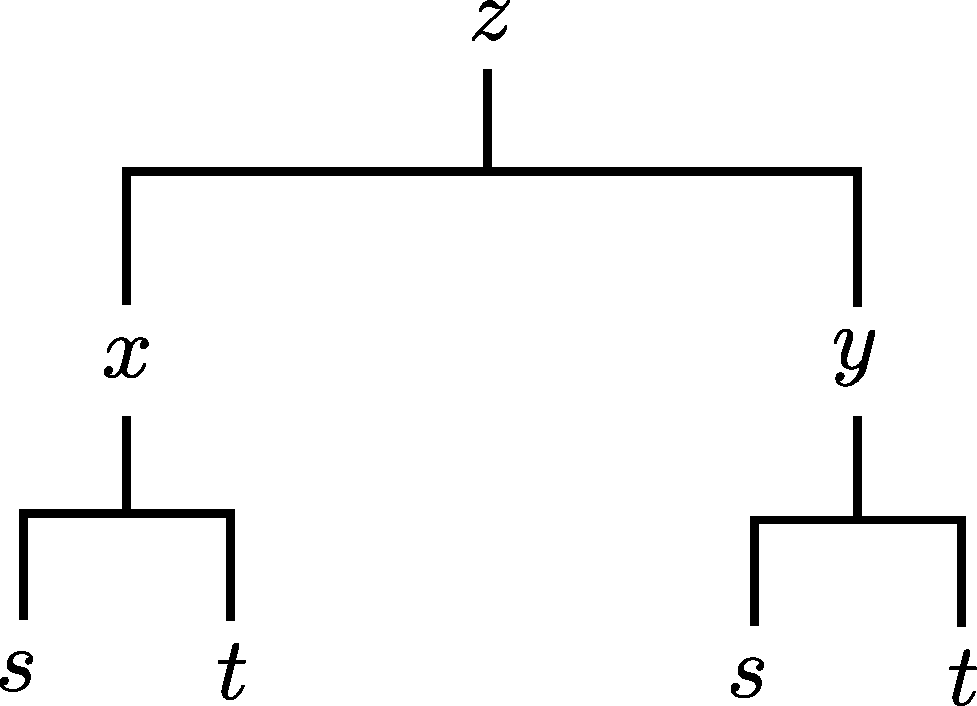
\includegraphics[width=0.35\linewidth]{chain2}
    \end{figure}
\end{frame}

\begin{frame}{Keðjuregla} 

\begin {block}{Ritháttur 6.\arabic{mycount}.}\stepcounter{mycount}
 Ritum $z=f(x,y)$ þar sem $x=x(s,t)$ og $y=y(s,t)$ eru föll af breytum $s$ og  $t$.  Þá er 
$$\begin{bmatrix}\frac{\partial z}{\partial s} 
& \frac{\partial z}{\partial t}\end{bmatrix}
=\begin{bmatrix}\frac{\partial z}{\partial x} 
& \frac{\partial z}{\partial y}\end{bmatrix}
\begin{bmatrix}\frac{\partial x}{\partial s} 
& \frac{\partial x}{\partial t}\\
\frac{\partial y}{\partial s} 
& \frac{\partial y}{\partial t}
\end{bmatrix}$$
\end{block}
 
\end{frame}

\begin{frame}{Keðjuregla} 

\begin {block}{Setning 6.\arabic{mycount}}\stepcounter{mycount}
Látum $u$ vera fall af $n$ breytum $x_1, x_2, \ldots, x_n$ þannig að hvert $x_i$ má rita sem fall af $m$ breytum $t_1, t_2, \ldots, t_m$.  Gerum ráð fyrir að allar hlutafleiðurnar $\frac{\partial u}{\partial x_i}$ og $\frac{\partial x_i}{\partial t_j}$ séu til og samfelldar.  Þegar $u$ er skoðað sem fall af breytunum $t_1, t_2, \ldots, t_m$ fæst að 
$$\frac{\partial u}{\partial t_j}=
\frac{\partial u}{\partial x_1}\frac{\partial x_1}{\partial t_j}
+\frac{\partial u}{\partial x_2}\frac{\partial x_2}{\partial t_j}
+\cdots+
\frac{\partial u}{\partial x_n}\frac{\partial x_n}{\partial t_j}.$$
\end{block}
\begin{figure}[h!]
           \centering
            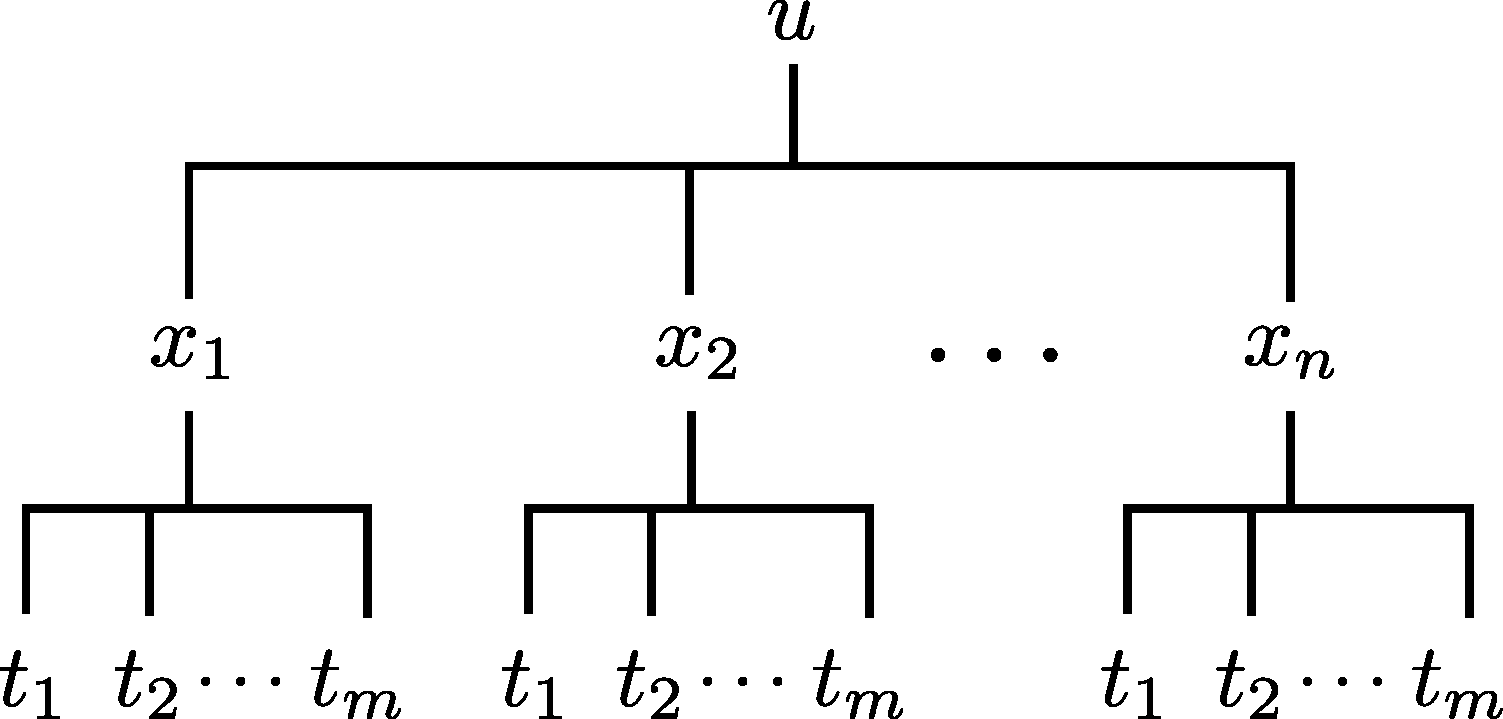
\includegraphics[width=0.45\linewidth]{chain3}
    \end{figure}
\end{frame}

\begin{frame}{Keðjuregla} 

\begin {block}{Dæmi 6.\arabic{mycount}}\stepcounter{mycount}
Látum $T$ vera fall af fall af $x$, $y$ og $t$, og $x$ og $y$ föll af $t$. Finnum $\frac{ dT}{dt}$.
\end {block}
\begin{figure}[h!]
           \centering
            \includegraphics[width=0.35\linewidth]{chain5}
    \end{figure}
$$\frac{d T}{d t} = \frac{\partial T}{\partial x} \frac{d x}{d t} +\frac{\partial T}{\partial y} \frac{d y}{\partial t} + \frac{\partial T}{\partial t} .$$
\end{frame}

\begin{frame}{Keðjuregla} 

\begin {block}{Dæmi 6.\arabic{mycount}}\stepcounter{mycount}
Látum $T$ vera fall af fall af $x$, $y$, $s$ og $t$, og $x$ og $y$ föll af $s$ og $t$. Finnum $\frac{ \partial T}{\partial t}$.
\end {block}
\begin{figure}[h!]
           \centering
            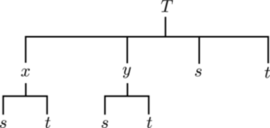
\includegraphics[width=0.45\linewidth]{chain6}
    \end{figure}
$$\frac{\partial T}{\partial t} = \frac{\partial T}{\partial x} \frac{\partial x}{\partial t} +\frac{\partial T}{\partial y} \frac{\partial y}{\partial t} + \left(\frac{\partial T}{\partial t}\right)_{x,y,s} .$$
\end{frame}

\begin{frame}{Keðjuregla} 

\begin {block}{Dæmi 6.\arabic{mycount}}\stepcounter{mycount}
Látum $z$ vera fall af fall af $u$, $v$ og $r$, $u$ og $v$ vera föll af $x$, $y$ og $r$ og $r$ vera fall af $x$ og $y$. Skrifum niður $\frac{\partial z}{\partial x}$.
\end {block}
\begin{figure}[h!]
           \centering
            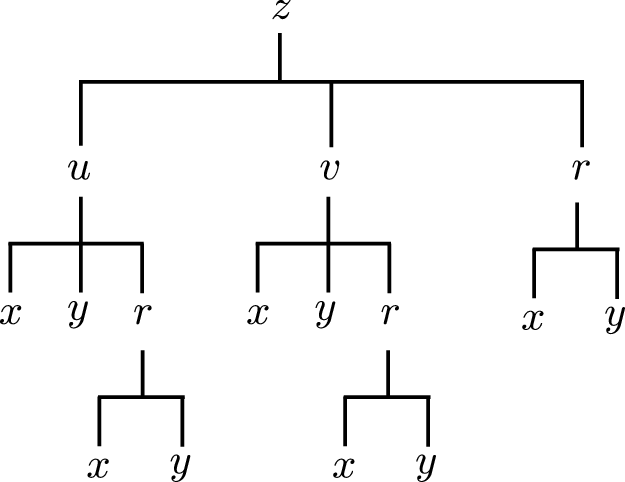
\includegraphics[width=0.45\linewidth]{chain4}
    \end{figure}
$$\frac{\partial z}{\partial x} = \frac{\partial z}{\partial u} \frac{\partial u}{\partial x} +\frac{\partial z}{\partial u} \frac{\partial u}{\partial r} \frac{\partial r}{\partial x} 
+ \frac{\partial z}{\partial v} \frac{\partial v}{\partial x} + \frac{\partial z}{\partial v} \frac{\partial v}{\partial r} \frac{\partial r}{\partial x} +\frac{\partial z}{\partial r} \frac{\partial r}{\partial x}.$$
\end{frame}



\begin{frame}{Jákvætt einsleit föll} 

\begin {block}{Skilgreining 6.\arabic{mycount}}\stepcounter{mycount}

Fall $f(x_1, x_2, \ldots, x_n)$ er sagt vera {\em jákvætt einsleitt af stigi $k$} (e.~positively homogeneous of degree $k$) ef fyrir sérhvern punkt $(x_1, x_2, \ldots, x_n)$ og sérhverja tölu $t>0$ gildir að 
$$f(tx_1, tx_2, \ldots, tx_n)=t^kf(x_1, x_2, \ldots, x_n).$$
\end{block}

\end{frame}



\begin{frame}{Jákvætt einsleit föll} 

\begin {block}{Setning 6.\arabic{mycount}}\stepcounter{mycount}
 Ef fall $f(x_1, x_2, \ldots, x_n)$ hefur samfelldar fyrsta stigs hlutafleiður og er jákvætt einsleitt af stigi $k$ þá er 
$$\sum_{i=1}^n x_if_i(x_1, x_2, \ldots, x_n)=kf(x_1, x_2, \ldots, x_n).$$ 
 \end{block}

\end{frame}

\end{document}